% 吡啶应用和补氢后的结果，接在读者检查步骤之后。
\begin{figure}[H]
\centering
% 原图3024×1758；几何范围(900,370,2120,1680)，1220×1310；70mm约443ppi。
% 不包含摘要；当前会话保留骨架多重度的现象由第7章正文另行说明。
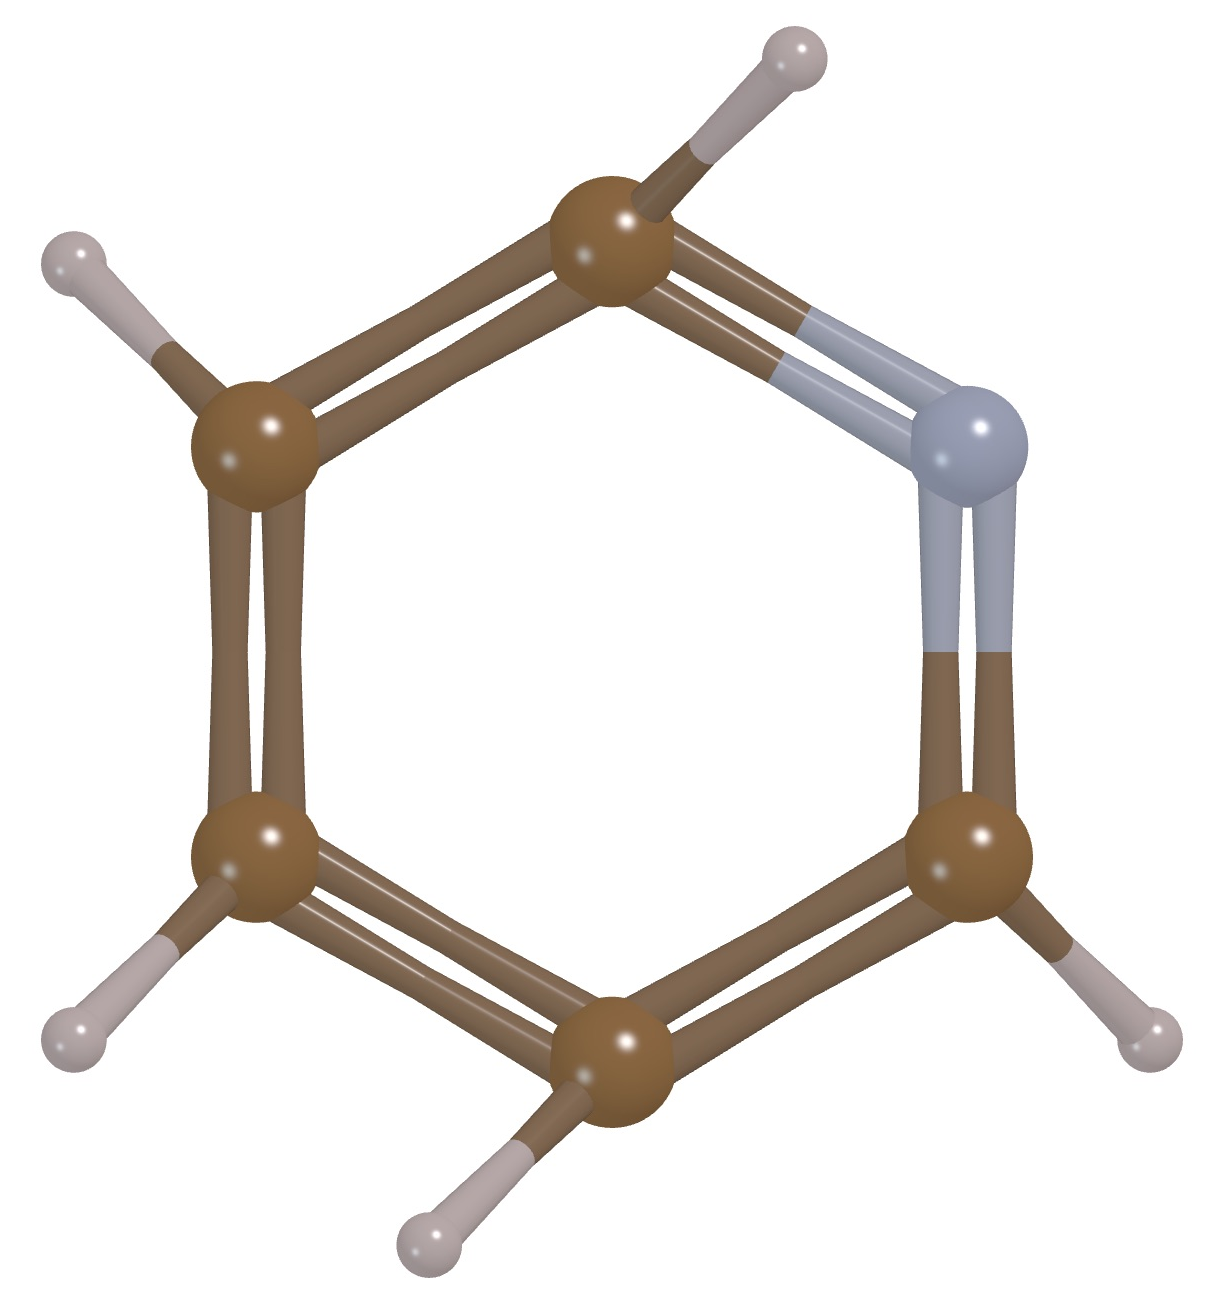
\includegraphics[width=70mm]{publication-assets/crop-60c8057a2bb7c31f0fd8.png}
\caption{Online中完成元素替换并对六个环原子补氢后的实际几何：五个碳、一个氮和五个氢，共11个原子、11条连接。此图未经过几何优化；继续计算时，使用随书\file{pyridine.json}中已修正的中性单重态参考结构。}
\label{fig:pyridine-built-model}
\end{figure}
